\documentclass[11pt]{article}
\usepackage[a4paper,margin=22mm,headheight=16pt]{geometry}
\usepackage{fontspec,xeCJK,xcolor,graphicx,enumitem,fancyhdr,titlesec}
\usepackage{hyperref}
\IfFontExistsTF{Times New Roman}{\setmainfont{Times New Roman}}{\setmainfont{TeX Gyre Termes}}
\IfFontExistsTF{FangSong}{\setCJKmainfont[AutoFakeBold=2]{FangSong}}{\IfFontExistsTF{仿宋}{\setCJKmainfont[AutoFakeBold=2]{仿宋}}{\IfFontExistsTF{FandolFang-Regular.otf}{\setCJKmainfont[AutoFakeBold=2]{FandolFang-Regular.otf}}{\setCJKmainfont{FandolSong-Regular.otf}}}}
\definecolor{ink}{HTML}{173747}\definecolor{accent}{HTML}{227E82}
\hypersetup{colorlinks=true,urlcolor=accent,linkcolor=accent}
\linespread{1.22}\setlength{\parindent}{0pt}\setlength{\parskip}{6pt}
\setlist[itemize]{leftmargin=1.4em,itemsep=3pt}
\titleformat{\section}{\large\bfseries\color{ink}}{}{0pt}{}
\titlespacing*{\section}{0pt}{14pt}{7pt}
\pagestyle{fancy}\fancyhf{}\lhead{\small OMNI LEARNING / 学习手册}\rhead{\small Source-grounded learning}\cfoot{\small\thepage}
\emergencystretch=2em\widowpenalty=10000\clubpenalty=10000
\newcommand{\Needspace}[1]{\par\begingroup\dimen0=#1\relax\vskip0pt plus\dimen0\penalty-100\vskip0pt plus-\dimen0\vskip\dimen0\penalty9999\vskip-\dimen0\vskip0pt\endgroup}
\begin{document}


{\LARGE\bfseries\color{ink} 永乐宫城与皇权表达}\par

2026-10-08 | Day03/30 | 阅读 8 分钟 + 练习 3 分钟\par\vspace{6pt}

\Needspace{5\baselineskip}\section*{今日导航}

今天回答：宫殿的轴线和尺度，能告诉我们多少政治信息？目标是把建筑作为历史材料，同时理解其证据边界。先回忆昨天的双栏：政治权威的表达与具体事务的处理，可能通过不同空间呈现。

\Needspace{5\baselineskip}\section*{先确认地点与时间}

UNESCO 的遗产说明指出，北京紫禁城由明成祖朱棣在1406年至1420年间营建，并经历后续明清时期的长期使用。[S3] 这给我们一个时间锚点，但今天看到的每个构件未必都原封不动来自最初营建。遗产是持续使用、修缮和解释的结果，观察时要区分建筑群的建立与某个部位的年代。

\begin{center}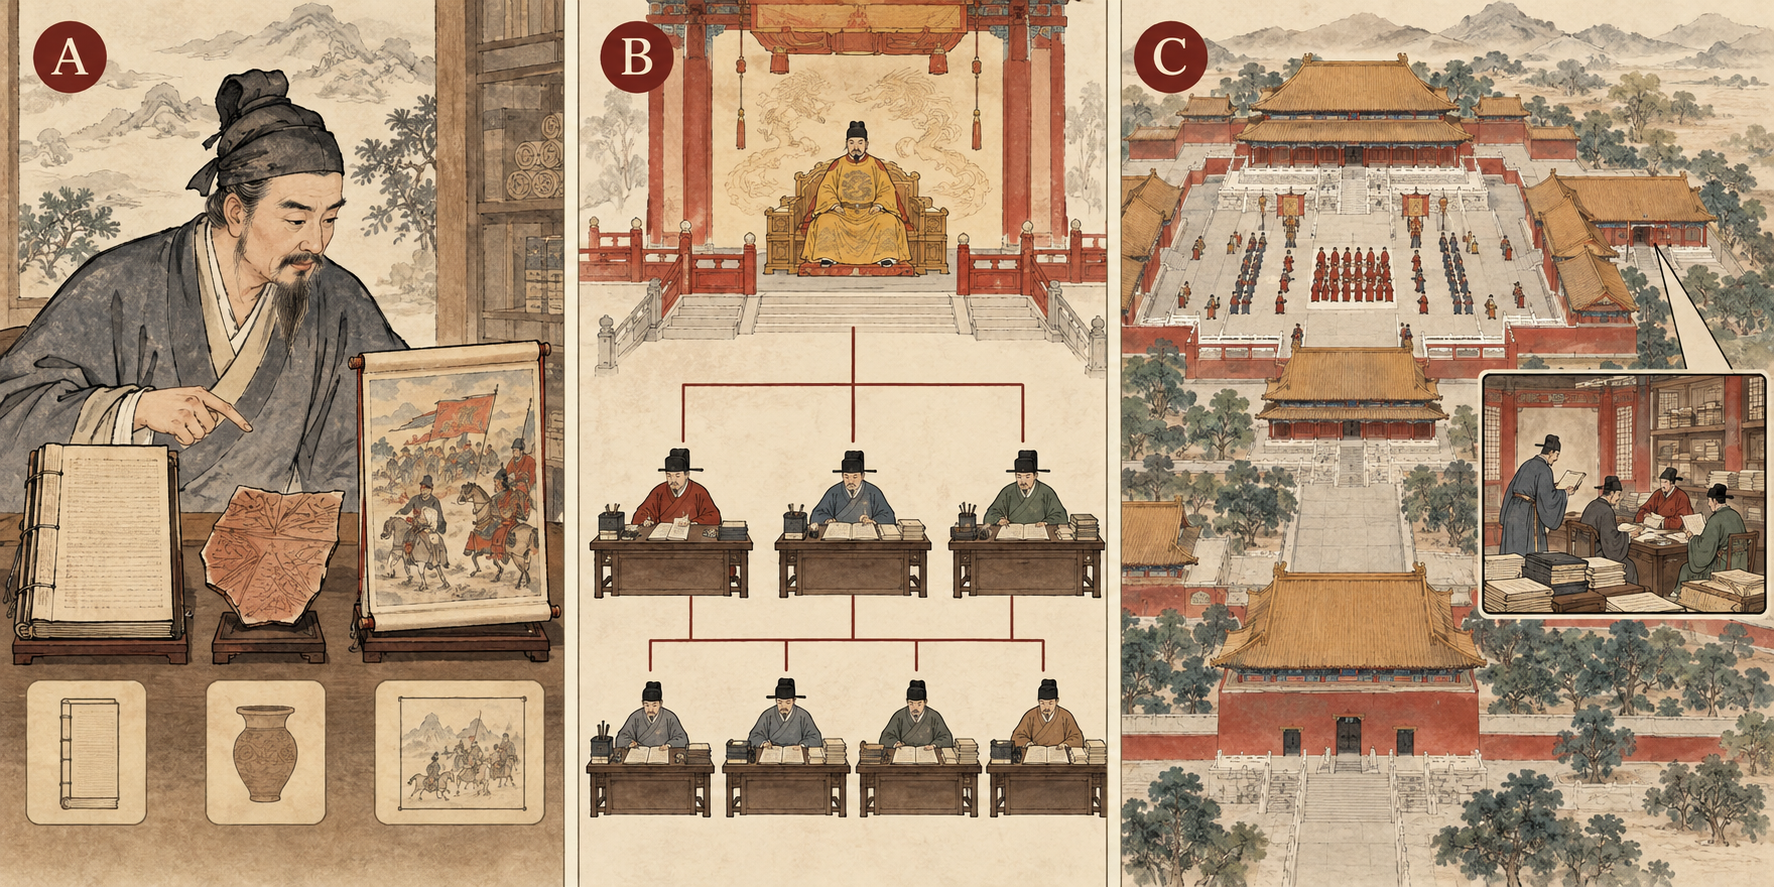
\includegraphics[width=\linewidth,height=0.26\textheight,keepaspectratio]{../assets/figure-e75918c40f59.png}\par

{\small 本课重点看 C 区。A 文字、器物与图像需要互证；B 思考决策和执行关系；C 区分宫城礼仪空间与日常政务。人物、服饰和机构排列均非史料复原。}\par

{\footnotesize AI生成教学示意，非实物照片、原始史料或官方架构。生成方式：内置文生图；提示词见仓库 docs/image-prompts.json。}\end{center}

\Needspace{5\baselineskip}\section*{空间怎样表达秩序}

中央轴线、对称布局、前朝后寝等安排，可以引导行进并组织礼仪与生活空间；这些是 UNESCO 说明中提到的特征。[S3] 它们让某种等级和秩序可被感知，但不能仅凭布局就推断每一次真实政治互动。

图 C 用抽象宫城和处理文书的场景作对照。前者提醒我们观察公开礼仪，后者提醒日常治理还涉及信息、协商与执行。图中的人物、具体建筑和办公方式均为教学想象，不是永乐时期复原，不可作为独立历史证据。

明清陵寝材料也能帮助观察皇权如何在另一种空间中表达。[S4] 宫殿与陵寝用途不同，比较时应找共同问题，如路线、等级和纪念，而不是假定它们只有同一种功能。

\Needspace{5\baselineskip}\section*{三层观察，不跳过中间环节}

第一层记录可见事实：主要轴线在哪里，建筑与院落如何排列。第二层结合可靠说明解释用途与礼仪关系。第三层才提出更大的政治问题：这种安排怎样表达统治者希望被理解的秩序？第三层属于解释，需要说明依据。

教学反例：“宫殿很大，因此皇帝能有效控制所有地方。”建筑规模可能表明资源动员和象征意图，却不足以直接证明地方治理效果。要研究后者，需要财政、行政、交通和地方实践等材料。艺术与建筑不是无用，它们提供的是有边界的证据。

\Needspace{5\baselineskip}\section*{三分钟练习与自查}

为一张宫殿照片写两句可以由照片支持的观察，再写一句必须借助其他材料才能回答的问题。

参考观察：“建筑沿一个主要方向排列”“前后院落形成多次进入的门槛”。问题：“哪些人能在何种仪式下进入这些空间？”自查有没有把想象的礼仪动作直接写成照片里的事实。若照片裁切范围很小，应承认无法看见全局。可选读原址说明，今天不要求记殿名清单。

\Needspace{5\baselineskip}\section*{复盘与明日连接}

建筑既是物质空间，也是政治文化的表达；它能帮助提问，却不能替代全部政治史证据。前两课学到的时间线与制度分析，现在多了一种材料视角。明天回到政治事件，学习靖难之役与继承问题，并继续区分事实、立场和后世叙述。

\Needspace{6\baselineskip}\section*{扩展学习 / Further reading}\small 以下为选读，不计入每日必做时间。\begin{enumerate}[leftmargin=1.6em]

\item [S1] \href{https://www.metmuseum.org/essays/ming-dynasty-1368-1644}{Ming Dynasty (1368–1644)} — 从文物与艺术观察明代，避免把宫廷与文人经验视为全部社会。\par The Metropolitan Museum of Art | 发布：2002-10-01 | 核验：2026-10-08

\item [S2] \href{https://www.dpm.org.cn/court/system/236406.html}{中书省} — 核对洪武时期机构调整，并把制度事实与作者的因果解释区分开。\par 故宫博物院 | 发布：未标注 | 核验：2026-10-08

\item [S3] \href{https://whc.unesco.org/en/list/439/}{Imperial Palaces of the Ming and Qing Dynasties} — 查看北京宫殿营建时间、轴线与礼仪空间；注意明清长期改建。\par UNESCO | 发布：未标注 | 核验：2026-10-08

\item [S4] \href{https://whc.unesco.org/en/list/1004/}{Imperial Tombs of the Ming and Qing Dynasties} — 从陵寝空间理解皇权表达，与宫殿材料交叉观察。\par UNESCO | 发布：未标注 | 核验：2026-10-08

\item [S5] \href{https://www.metmuseum.org/exhibitions/listings/2009/arts-of-the-ming-dynasty}{Arts of the Ming Dynasty} — 旧展览档案用于认识作品种类，不代表展览仍在开放。\par The Metropolitan Museum of Art | 发布：未标注 | 核验：2026-10-08

\end{enumerate}

\end{document}